\documentclass[runningheads]{llncs}

\usepackage{graphicx}
\usepackage{booktabs}
\usepackage{amsmath}

\begin{document}

\title{Artist-Conditional Lyric Generation\\with QLoRA Adapter Blending}

\author{Ali \"Ozkaya}
\institute{Department of Computer Engineering,\\Izmir Institute of Technology\\
\email{aliozkaya@std.iyte.edu.tr}}

\maketitle

\begin{abstract}
We present a pipeline for artist-conditional lyric generation using per-artist QLoRA adapters on a quantized Gemma~4 E4B model. One low-rank adapter is trained per artist, and we propose inference-time linear blending of adapter weights for style interpolation. We select five progressive metal artists whose lyrics are thematically similar, forcing the model to capture fine-grained stylistic differences rather than genre-level features. A RoBERTa-based artist-attribution classifier achieves 92.2\% accuracy on held-out lyrics and serves as the primary evaluation instrument. We compare adapters against zero-shot and few-shot baselines, finding that LoRA adapters achieve 98.3\% and 86.3\% target-artist attribution for Gojira and Tool respectively, compared to 1.1\% and 97.1\% for zero-shot prompting. Ablation studies over adapter method (LoRA vs.\ DoRA) and rank ($r \in \{4, 8, 16\}$) are also presented.
\end{abstract}

\keywords{lyric generation \and QLoRA \and adapter blending \and parameter-efficient fine-tuning}

% ============================================================
\section{Introduction}
\label{sec:intro}

Large language models excel at open-ended text generation~\cite{radford2019language}, yet controlling stylistic properties remains challenging. In lyric writing, the output must reflect an artist's distinctive voice---their vocabulary, themes, and rhythmic patterns.

Parameter-efficient fine-tuning methods such as LoRA~\cite{hu2022lora} and QLoRA~\cite{dettmers2023qlora} enable adapting large models on consumer hardware by training only low-rank weight matrices. A natural extension is training one adapter per artist and combining them at inference time, as explored in adapter merging~\cite{huang2023lorahub} and adapter soup~\cite{chronopoulou2023adaptersoup}.

We apply this idea to lyric generation with the following contributions:
\begin{enumerate}
    \item A pipeline for per-artist QLoRA adapters on 4-bit quantized Gemma~4 E4B, using five same-genre artists as a deliberately challenging testbed.
    \item A RoBERTa-based artist-attribution classifier (92.2\% accuracy) as an automated evaluation instrument.
    \item Systematic comparison against zero-shot and few-shot baselines, with LoRA vs.\ DoRA and rank ablation studies.
    \item A proposal for inference-time adapter blending via linear weight interpolation.
\end{enumerate}

% ============================================================
\section{Related Work}
\label{sec:related}

\textbf{Parameter-Efficient Fine-Tuning.}
LoRA~\cite{hu2022lora} injects a trainable low-rank decomposition $\Delta W = BA$ while freezing pretrained weights. QLoRA~\cite{dettmers2023qlora} extends this with 4-bit NF4 quantization. DoRA~\cite{liu2024dora} decomposes weight updates into magnitude and direction components.

\textbf{Creative Text Generation.}
LLM-based creative generation spans poetry, storytelling, and songwriting~\cite{vonrutte2023language}. Fine-tuning for individual artist styles is less studied due to data requirements and evaluation difficulty.

\textbf{Adapter Composition.}
LoRAHub~\cite{zhang2023lorahub} learns composition coefficients across task-specific adapters; AdapterSoup~\cite{chronopoulou2023adaptersoup} averages adapter weights for generalization. We apply linear blending to interpolate between artist styles.

% ============================================================
\section{Methodology}
\label{sec:method}

\subsection{Pipeline Overview}

Our pipeline has four stages: (1)~preprocessing, (2)~classifier training, (3)~per-artist QLoRA adapter training, and (4)~inference with optional adapter blending. The classifier validates that real lyrics are distinguishable and later evaluates generated lyrics.

\subsection{Preprocessing}

Raw lyrics contain structural annotations (\texttt{[Verse~1]}, \texttt{[Chorus]}) that encode structure rather than style. We strip all bracketed headers and filter songs shorter than 100 characters.

\subsection{Artist-Attribution Classifier}

We fine-tune RoBERTa-base~\cite{liu2019roberta} for 5-class classification. The classifier serves as an evaluation instrument: high-confidence attribution to the target artist indicates successful style capture. We use a maximum sequence length of 512 tokens, covering 96.7\% of songs.

\subsection{QLoRA Adapter Training}

We use Gemma~4 E4B~\cite{gemma2025} (${\sim}$4B parameters, dense) loaded in 4-bit NF4 quantization with double quantization and bfloat16 compute via bitsandbytes~\cite{dettmers2022llmint8}. We chose the dense architecture over the 26B MoE variant because adapter blending assumes dense layers---merging LoRA weights across routed experts introduces ambiguity.

LoRA adapters ($r{=}8$, $\alpha{=}16$, dropout 0.1) target all attention ($q$, $k$, $v$, $o$) and MLP (gate, up, down) projections in the language model layers, selected via regex to exclude vision/audio encoder layers.

The training prompt \texttt{"Write song lyrics.\textbackslash n\textbackslash n\{lyrics\}"} is deliberately generic with no artist name, ensuring style is encoded in adapter weights---a prerequisite for clean blending.

\subsection{Adapter Blending}

At inference time, we linearly interpolate LoRA weights:
\begin{equation}
    \Delta W_{\text{blend}} = \sum_{i=1}^{N} \alpha_i \, \Delta W_i, \quad \sum_{i=1}^{N} \alpha_i = 1
\end{equation}
producing an adapter whose style lies between the constituent artists.

\subsection{Baselines}

\begin{itemize}
    \item \textbf{B1 -- Zero-shot:} Base model prompted with ``Write song lyrics in the style of \{artist\}.'' No fine-tuning; the artist name in the prompt is the only signal.
    \item \textbf{B2 -- Few-shot:} Same prompt augmented with 3 randomly sampled training lyrics as in-context examples.
\end{itemize}

Both baselines use identical generation parameters as the adapters (temperature 0.9, top-$p$ 0.9, repetition penalty 1.1, 200--512 tokens). We generate 10 samples per artist per method and report mean and standard deviation of classifier attribution. Crucially, baselines include the artist name in the prompt while adapters do not---adapters must encode style entirely in their weights.

% ============================================================
\section{Experimental Setup}
\label{sec:setup}

\subsection{Dataset and Artist Selection}

We use the \texttt{genius-lyrics-cleaned} dataset from Hugging Face (${\sim}$3.18M songs). We select five progressive/extreme metal artists: \textbf{Death} (116), \textbf{Gojira} (86), \textbf{Meshuggah} (116), \textbf{Opeth} (118), and \textbf{Tool} (74), totaling 510 songs after preprocessing.

Same-genre selection ensures evaluation validity: a cross-genre classifier would distinguish genre rather than individual style. Our five artists share a genre but differ in voice: Gojira's environmental philosophy, Tool's cryptic wordplay, Death's technical lyricism, Meshuggah's mechanical abstraction, and Opeth's poetic melancholy.

We apply stratified splitting: 459 training, 51 evaluation (90/10).

\subsection{Training Configuration}

\textbf{Classifier:} RoBERTa-base, 5 epochs, lr $2{\times}10^{-5}$, batch 8, weight decay 0.01, warmup ratio 0.1, best checkpoint by validation accuracy.

\textbf{QLoRA:} SFTTrainer (TRL), 3 epochs, batch 2 with gradient accumulation 2 (effective batch 4), lr $2{\times}10^{-4}$, cosine schedule, warmup ratio 0.1, weight decay 0.05, max length 512, gradient checkpointing. Trained on NVIDIA RTX 5090 (32\,GB).

\textbf{Generation:} Nucleus sampling, temperature 0.9, top-$p$ 0.9, repetition penalty 1.1, 200--512 tokens.

\subsection{Reproducibility}

All code, data splits, and notebooks are available at \url{https://github.com/raccoon-42/lora-lyrics} with step-by-step reproduction instructions.

% ============================================================
\section{Results}
\label{sec:results}

\begin{figure}[t]
    \centering
    \begin{minipage}[t]{0.48\textwidth}
        \centering
        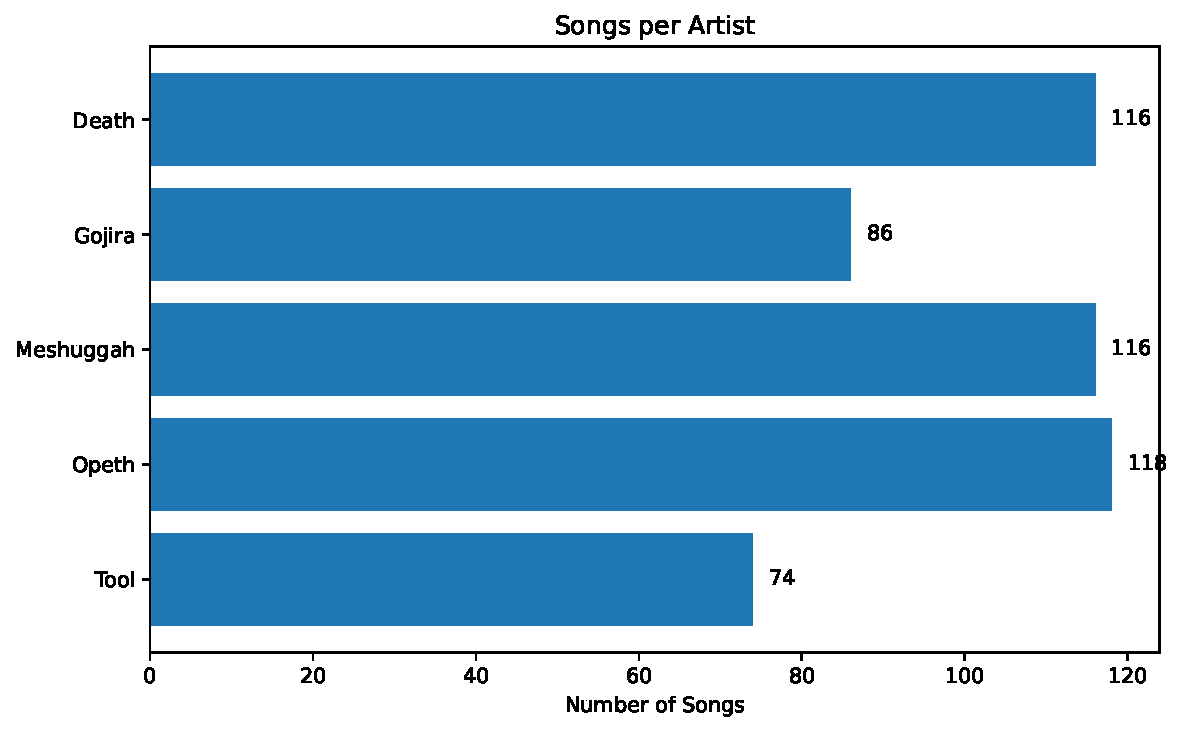
\includegraphics[width=\textwidth]{figures/artist_distribution.pdf}
        \caption{Songs per artist.}
        \label{fig:distribution}
    \end{minipage}
    \hfill
    \begin{minipage}[t]{0.48\textwidth}
        \centering
        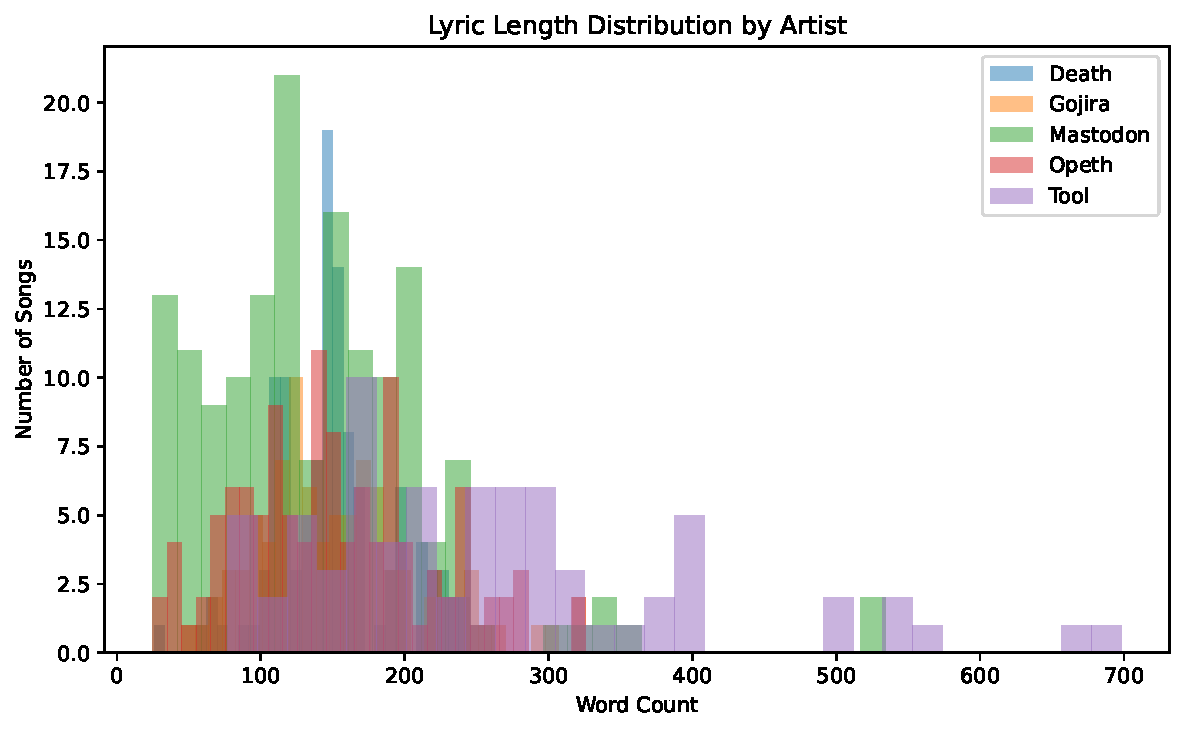
\includegraphics[width=\textwidth]{figures/lyric_lengths.pdf}
        \caption{Lyric length distributions.}
        \label{fig:lengths}
    \end{minipage}
\end{figure}

\subsection{Data Analysis}

Figure~\ref{fig:distribution} shows moderate class imbalance (Opeth has 1.6$\times$ Tool's songs). Token-level analysis reveals a median of 216 tokens per song (mean 238); only 17/510 (3.3\%) exceed 512 tokens (Figure~\ref{fig:lengths}).

\subsection{Classifier Results}

\begin{table}[t]
\centering
\caption{Per-class classifier performance on the evaluation set (51 songs). Overall accuracy: 92.2\%.}
\label{tab:classifier}
\begin{tabular}{lccc}
\toprule
\textbf{Artist} & \textbf{Precision} & \textbf{Recall} & \textbf{F1} \\
\midrule
Death     & 1.00 & 1.00 & 1.00 \\
Gojira    & 0.75 & 0.75 & 0.75 \\
Meshuggah & 1.00 & 0.92 & 0.96 \\
Opeth     & 0.92 & 1.00 & 0.96 \\
Tool      & 0.86 & 0.86 & 0.86 \\
\midrule
\textbf{Weighted avg} & \textbf{0.92} & \textbf{0.92} & \textbf{0.92} \\
\bottomrule
\end{tabular}
\end{table}

Table~\ref{tab:classifier} shows per-class results. Death is perfectly classified; Gojira is weakest (F1 = 0.75), confused with Opeth and Tool---consistent with their shared philosophical and environmental themes. A TF-IDF baseline achieves 82.4\% in 5-fold CV; the 10-point gain confirms RoBERTa captures deeper stylistic patterns.

\begin{figure}[t]
    \centering
    \begin{minipage}[t]{0.48\textwidth}
        \centering
        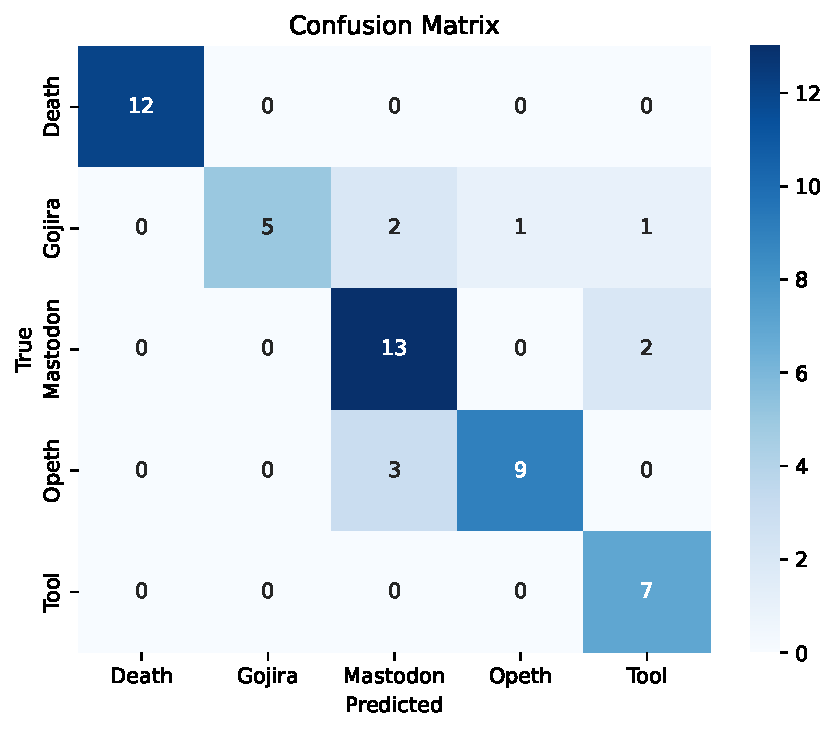
\includegraphics[width=\textwidth]{figures/confusion_matrix.pdf}
        \caption{Classifier confusion matrix.}
        \label{fig:confusion}
    \end{minipage}
    \hfill
    \begin{minipage}[t]{0.48\textwidth}
        \centering
        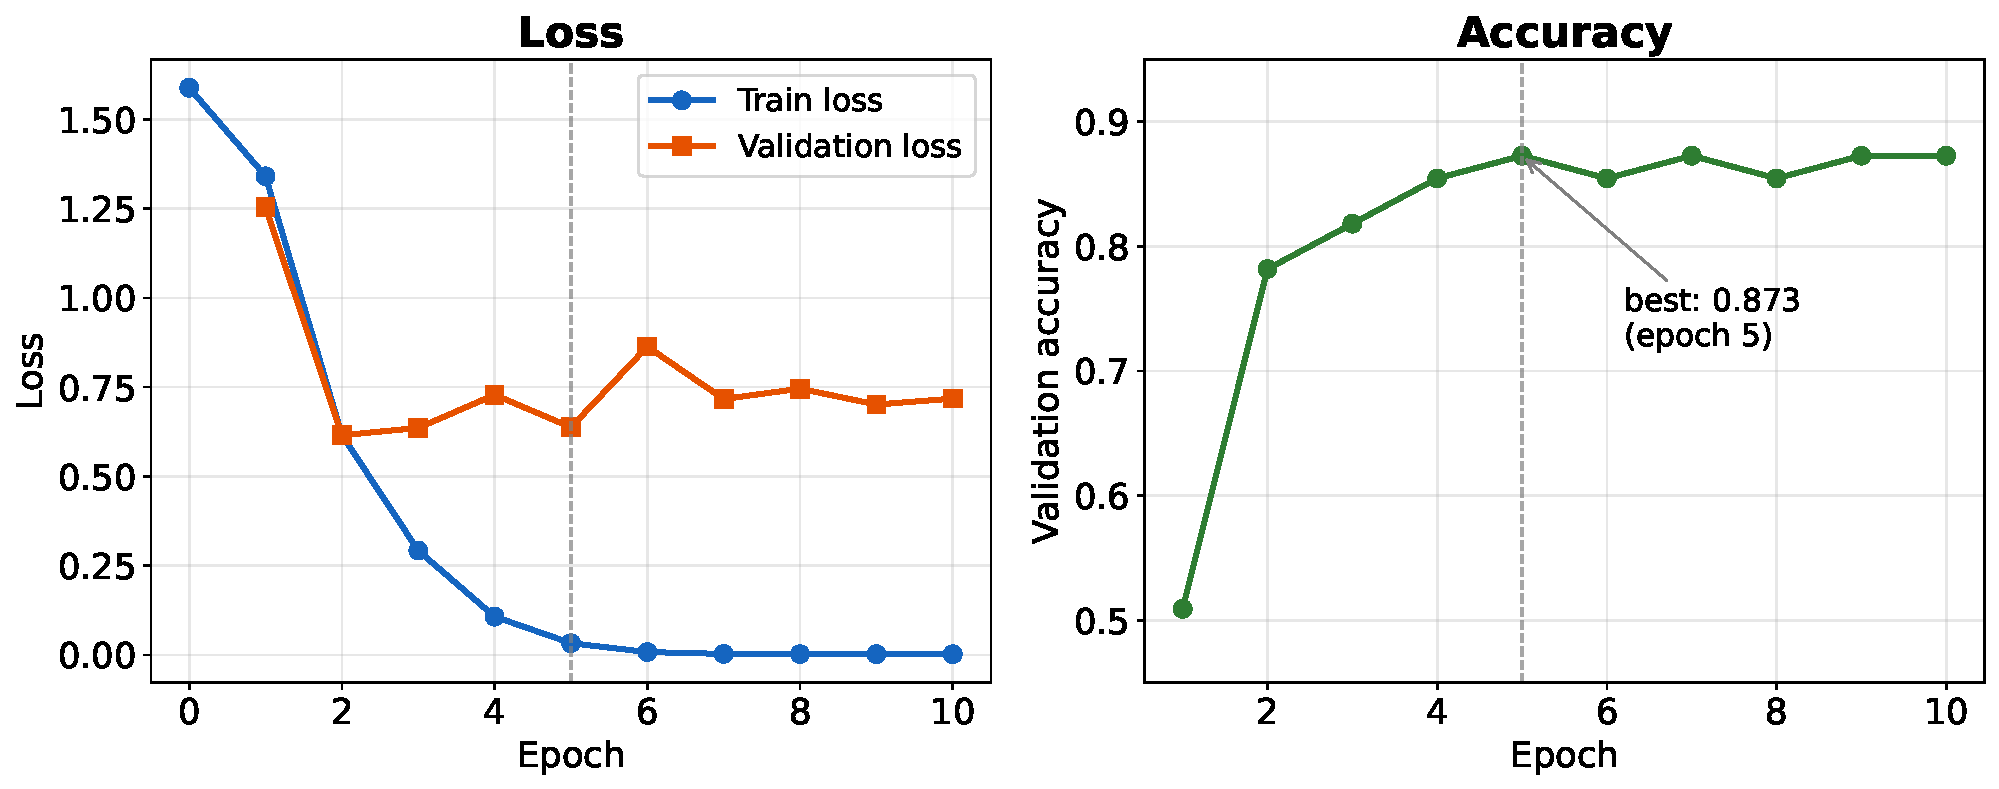
\includegraphics[width=\textwidth]{figures/training_curves.pdf}
        \caption{Loss and accuracy curves.}
        \label{fig:curves}
    \end{minipage}
\end{figure}

Figure~\ref{fig:confusion} shows that Gojira's errors split between Opeth and Tool (1 each); Meshuggah and Tool each lose one sample to Gojira. Figure~\ref{fig:curves} shows validation loss plateauing after epoch~3 with continued training loss decrease, indicating mild overfitting.

\subsection{Baseline Results}

\begin{table}[t]
\centering
\caption{Target-artist attribution (mean $\pm$ std, $n{=}10$) for baselines and adapters. Higher is better.}
\label{tab:results}
\begin{tabular}{llcc}
\toprule
\textbf{Method} & \textbf{Type} & \textbf{Gojira} & \textbf{Tool} \\
\midrule
Zero-shot     & Baseline  & $0.011 \pm 0.008$ & $0.971 \pm 0.034$ \\
Few-shot (3)  & Baseline  & $0.083 \pm 0.235$ & $0.947 \pm 0.044$ \\
\midrule
LoRA $r{=}8$  & Adapter   & $\mathbf{0.983 \pm 0.010}$ & $\mathbf{0.863 \pm 0.173}$ \\
DoRA $r{=}8$  & Adapter   & $0.989 \pm 0.002$ & $0.772 \pm 0.343$ \\
\bottomrule
\end{tabular}
\end{table}

Table~\ref{tab:results} and Figure~\ref{fig:comparison} present the main results. For Gojira, both baselines fail entirely: zero-shot achieves only 1.1\% attribution, and few-shot reaches 8.3\% with very high variance ($\sigma{=}0.235$). The LoRA adapter achieves 98.3\% with tight variance, a qualitative leap. For Tool, baselines score high (94.7--97.1\%) because the base model's default output style is classified as Tool by the classifier. The LoRA adapter scores 86.3\%, seemingly lower, but this reflects genuine stylistic specificity rather than a default bias.

\begin{figure}[t]
    \centering
    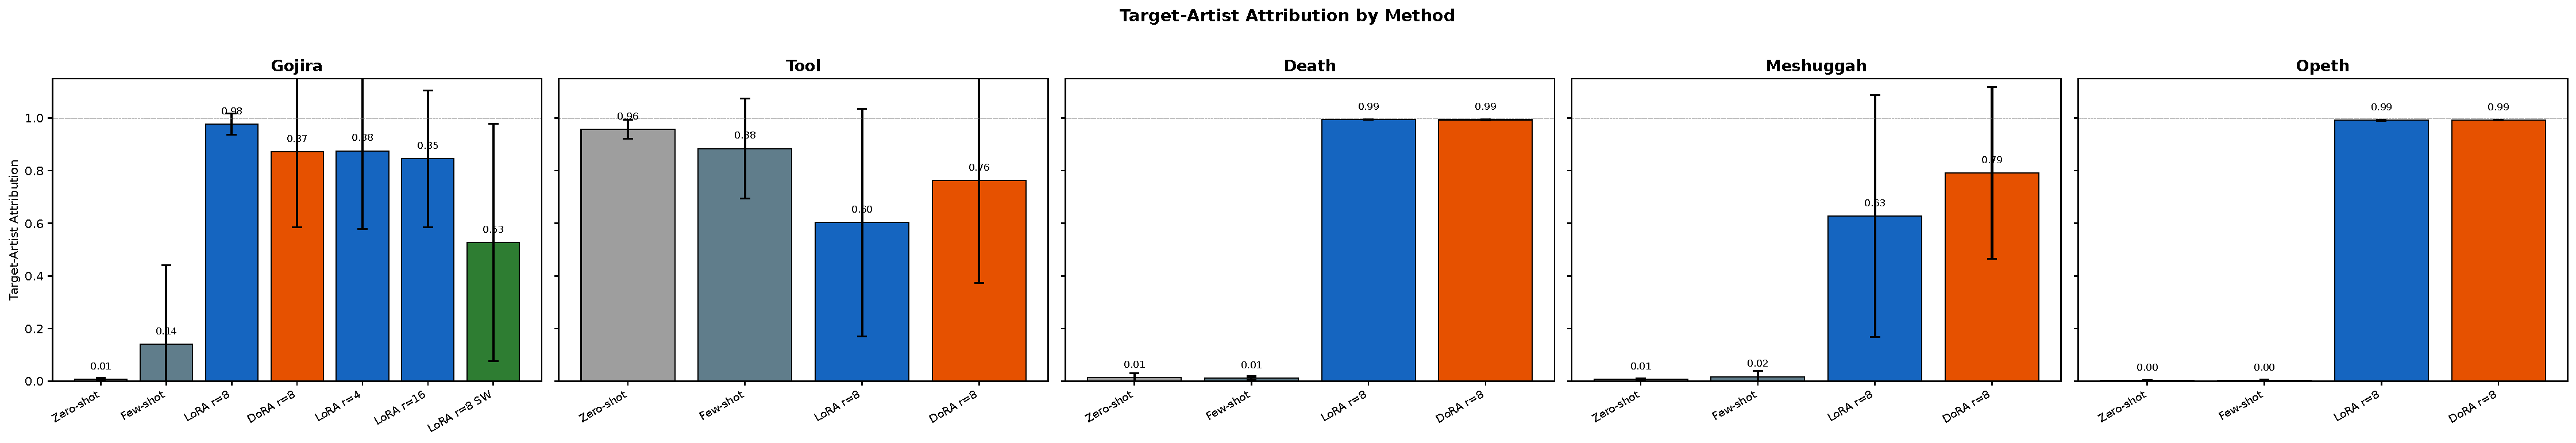
\includegraphics[width=0.85\textwidth]{figures/method_comparison.pdf}
    \caption{Target-artist attribution across all methods. Error bars show $\pm 1\sigma$ over 10 samples.}
    \label{fig:comparison}
\end{figure}

\subsection{Ablation Studies}

\begin{table}[t]
\centering
\caption{Ablation results (target-artist attribution, mean $\pm$ std, $n{=}10$).}
\label{tab:ablation}
\begin{tabular}{lcc}
\toprule
\textbf{Configuration} & \textbf{Gojira} & \textbf{Tool} \\
\midrule
\multicolumn{3}{l}{\textit{LoRA vs.\ DoRA ($r{=}8$)}} \\
LoRA  & $0.983 \pm 0.010$ & $\mathbf{0.863 \pm 0.173}$ \\
DoRA  & $\mathbf{0.989 \pm 0.002}$ & $0.772 \pm 0.343$ \\
\midrule
\multicolumn{3}{l}{\textit{Rank ablation (Gojira, LoRA)}} \\
$r{=}4$  & $0.881 \pm 0.275$ & -- \\
$r{=}8$  & $\mathbf{0.983 \pm 0.010}$ & -- \\
$r{=}16$ & $0.956 \pm 0.105$ & -- \\
\bottomrule
\end{tabular}
\end{table}

\textbf{LoRA vs.\ DoRA.}
On Gojira, DoRA marginally outperforms LoRA (98.9\% vs.\ 98.3\%) with lower variance. On Tool, LoRA is more stable (86.3\% vs.\ 77.2\%, $\sigma$ 0.17 vs.\ 0.34). The mixed results suggest neither method is uniformly superior at this scale.

\textbf{Rank ablation.}
Table~\ref{tab:ablation} and Figure~\ref{fig:ablation} show the effect of LoRA rank on Gojira. Rank $r{=}8$ is the sweet spot (98.3\%), with $r{=}4$ dropping to 88.1\% due to insufficient capacity and $r{=}16$ slightly degrading to 95.6\% with higher variance, possibly from overfitting on the small training set (86 songs).

\begin{figure}[t]
    \centering
    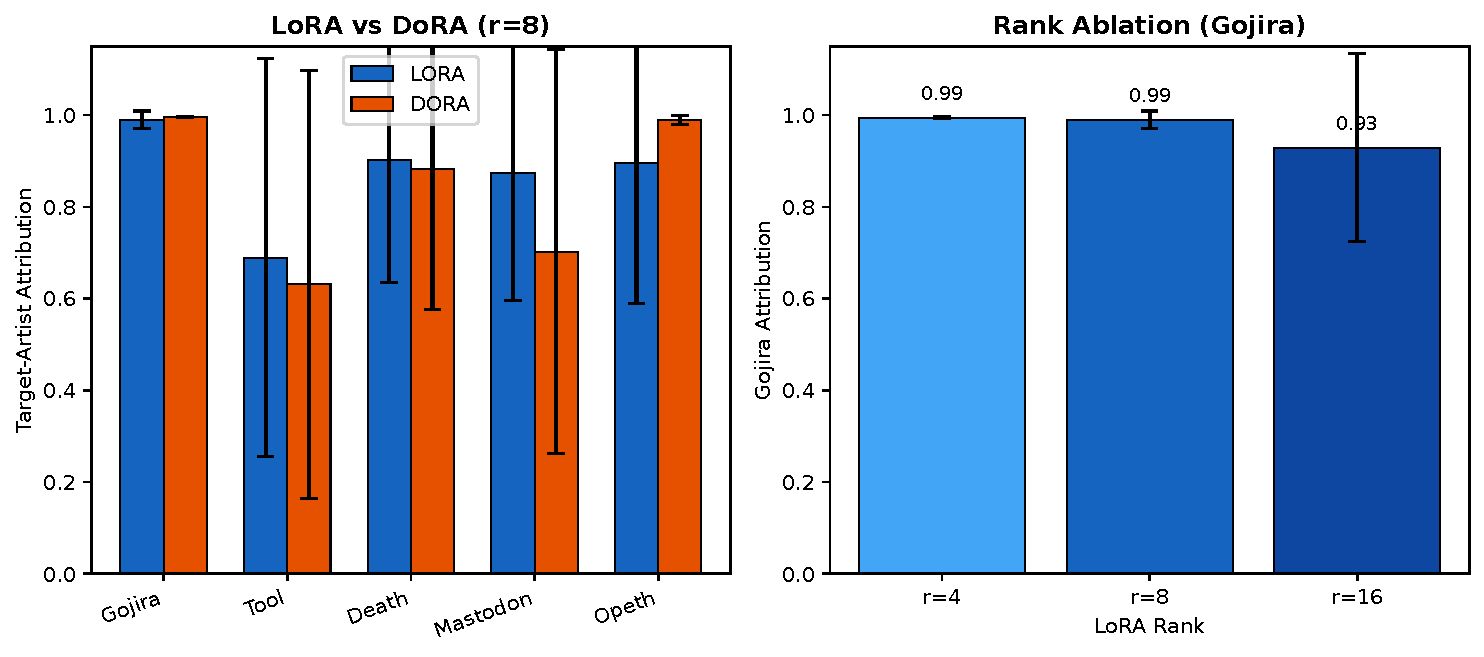
\includegraphics[width=0.85\textwidth]{figures/ablation.pdf}
    \caption{Left: LoRA vs.\ DoRA comparison ($r{=}8$). Right: Rank ablation for Gojira (LoRA).}
    \label{fig:ablation}
\end{figure}

% ============================================================
\section{Error Analysis}
\label{sec:error}

\textbf{Classifier errors.}
Gojira's low F1 (0.75) reflects genuine thematic overlap with Opeth (nature, existential reflection) and Tool (philosophical abstraction). The 92.2\% accuracy means ${\sim}$1 in 13 real songs is misclassified, a limitation that propagates into evaluation of generated lyrics.

\textbf{Tool baseline inflation.}
The base model's default generation style is consistently classified as Tool (94.9--97.1\%), even when prompted for Gojira. This inflates Tool's baseline scores and makes adapter improvements for Tool harder to demonstrate via attribution alone. The adapters produce more stylistically specific text, but occasional samples that deviate from Tool's narrow patterns get misclassified.

\textbf{Generation quality.}
Gojira adapter output captures environmental and philosophical themes (``roots of life'', ``giants living deep inside of us''). Tool output exhibits sardonic, confrontational tone. However, Tool's hallmarks---complex meter shifts, esoteric/Jungian references---are absent, suggesting finer signatures require more data. The $r{=}4$ and $r{=}16$ ablations show high variance (0.275 and 0.105), with some samples failing to capture the target style---consistent with the small training set (86 songs).

% ============================================================
\section{Discussion}
\label{sec:discussion}

\textbf{Evaluation methodology.}
Standard reference-based metrics (BLEU, ROUGE) are inapplicable to open-ended creative generation without ground-truth references. Classifier attribution directly measures style capture, but risks circularity: the classifier may learn superficial patterns that adapters also exploit. The Tool baseline inflation (97.1\% without fine-tuning) illustrates this. Perplexity and human evaluation are planned as complementary metrics.

\textbf{Data scale.}
With 74--86 training songs per artist, the rank ablation suggests $r{=}8$ is near-optimal, with higher ranks overfitting. No verbatim copying was observed.

\textbf{Remaining work.}
Adapter blending across artist pairs at $\alpha \in \{0.0, 0.25, 0.5, 0.75, 1.0\}$; perplexity evaluation; extension to remaining artists.

\textbf{Ethical considerations.}
Training on copyrighted lyrics is limited to academic research. The adapters could impersonate an artist's voice, raising authenticity and IP concerns. Metal lyrics may contain violent imagery that a fine-tuned model could amplify. Generated text may also hallucinate content falsely attributable to an artist.

% ============================================================
\section{Conclusion}
\label{sec:conclusion}

We presented a pipeline for artist-conditional lyric generation using per-artist QLoRA adapters on Gemma~4 E4B. A RoBERTa classifier (92.2\% accuracy) confirms that five same-genre metal artists are distinguishable. LoRA adapters massively outperform zero-shot and few-shot baselines for Gojira (98.3\% vs.\ 1.1\% and 8.3\% attribution), demonstrating that prompting alone cannot steer artist-specific style. Ablation studies show $r{=}8$ as optimal rank and mixed results for LoRA vs.\ DoRA. The Tool results highlight a limitation of single-metric evaluation: baseline inflation from the classifier's default bias. Future work includes adapter blending experiments, perplexity evaluation, and extension to the remaining three artists.

\bibliographystyle{splncs04}
\bibliography{references}

\end{document}
